\section{System Overview}
This section describes our system for robot sewing with a curved needle. Our system is consisted with two Kuka 7 d.o.f robots: one robot to manipulate the needle, i.e. piercing and one to control the fabric tube. The robot manipulating the needle is mounted with a motorized needle driver and the one controlling the fabric is mounted with a mandrel. This mandrel is placed inside the fabric tube to bound it tightly with the stent (Figure~\ref{fig:mandrel}). To ensure the the stent graft quality, each stitch is required to be at the correct place and have the correct length. We use a vision system to guide the robot movements in order to maintain the accuracy. The needle position is tracked during the whole task. The robot movements are first learned from human hand stitch demonstrations and then regenerated online to deliver the needle to stitch at the correct spot.

%We adopt an bimanual sewing approach: the curved needle is first carried by one robot (A) to pierce the fabric, and picked up by another robot (B) from the other side. The needle is then pulled out by the robot B and passed back to the robot A. The third robot moves to the next stitch position. These movements complete one cycle and repeat the cycle until the whole stent is sewed.


\subsection{Hardware design}

%------------- Curved needle  --------------
A surgical curved needle is used in our task to perform sewing (Figure~\ref{fig:setup}). It is manipulated by a surgical needle driver. This needle driver is widely used in laparoscopic surgery and is specially designed to hold firmly the needle.
%------------- Needle driver  --------------
%The motorized needle driver mounted on the robot is shown as Fig.1. This device incorporates a medical used Mayo Hager needle driver.
In our system, the needle driver is motorized for the robot to drive it (Figure~\ref{fig:needledriver}). This design has two set of constraints/guiding slots working in conjunction with pins. The linear slot lies in the direction along the handle of the needle driver and the constraint slot is coaxial with the needle driver axis; therefore the motor rotation can be mapped to the open and close of the needle driver. To reduce frictions in driving this mechanism, bears are used. All the mechanical components are 3D printed.

%The design projective is that the needle driver can be controlled without mounting a motor directly on its rotation axis, which may impede the needle driver approaching the sewn object in some direction.

%One feature of this design is that the two jaws of the needle driver work in an unsynchronized way. In the situation that the needle driver is not fully open, the center line of the grasper is located near one jaw which may create difficulty in approaching a target point and grasp precisely. One method to solve this disadvantage is to replace the linear guiding slot with slot with a critical geometry.

\begin{figure}
\centering
{
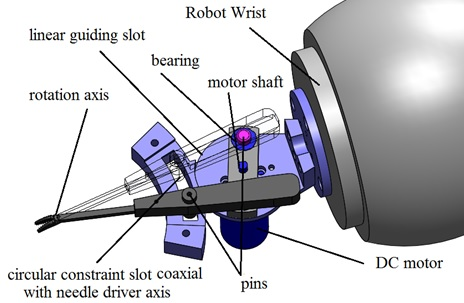
\includegraphics[width=7cm]{./fig/needledriver.jpg}
\caption{{Motorized needle driver}}
\label{fig:needledriver}}

\end{figure}

% --------------- Mandrel ----------------
Our mandrel is a 3D printed hollow cylinder to support the fabric. Its outer surface has groove for fixing stent and it supports the stent to tightly attache with the fabric. Slots are opened on the mandrel at the positions of stitches. They allow the needle to pierce in and out and hence sewing the stent on the fabric. An additional function of the slots is location marker: when illuminated from inside the mandrel, the location of the slots are visible, allowing us to identify the exact sewing positions.

\begin{figure}
\centering
{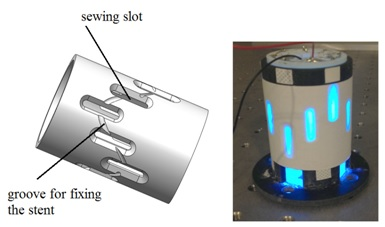
\includegraphics[width=8cm]{./fig/mandrel.jpg}
\caption{Mandrel}
\label{fig:mandrel}}
\end{figure}


\subsection{Learning from human demonstration}
With the current state of art, personalized stent grafts are hand sewn. This is because the delicate control of the needle is hard to programm to robotize. To tackle this problem, we adopt an learning for human demonstration approach for this task. Our learning starts by demonstrating to the robot multiple times how to make a stitch. The demonstrated motions are then segmented to different phases. A Gaussian Mixture Model (GMM)~\cite{cohn1996active} is used to encode each phases of the sewing motion and the generalised motion is then retrieved via Gaussian Mixture Regression (GMR). Generally speaking, this learning process involves the following steps:

\begin{enumerate}
\item{1}: Human demonstration of sewing
\item{2}: Motion segmentation
\item{3}: Primitive motions learning
\end{enumerate}

\subsubsection{Human demonstration of sewing}
The first step is to recode the stitching motion from human demonstrations. Human single side hand sewing motion involves a couple of stages including 1) needle approaching fabric, 2) needle piercing in, 3) releasing needle end 4)griping the needle tip and 5) pulling the needle out, 6) passing the needle to another hand and 7) picking up the needle head. At the beginning of the task, the needle driver grip firming the needle end. When the tip of the curved needle pierces out from the bottom of the fabric, the needle driver release the needle. The needle is remained in the same pose by the friction of the fabric. The needle driver is then approach the tip of the needle, and grip the tip. The needle then being pulled out from the fabric. Once the needle is completely pulled out from the fabric, the needle driver pass it to another fixed needle driver to re-grip the needle head. After re-griping, the needle driver move back to the starting position and finish a full circle of one stitch.

We use the kinesthetic teaching method to demonstrate all these stages to the robot. The robot is put in gravity compensation mode and its movement is guided by human. The needle driver open and close is controlled an electronic footpedal. The movement of the robot, as well as the needle driver status, i.e. open and close, are recorded. During the demonstrations, when the needle driver is close, we assume the needle is firmly connected with the driver and hence no slip between the needle and the driver will occur. Hence, during the demonstrations, we presume the relative pose between the needle and the driver is a constant value. At the beginning of each demonstration, we place the needle in an optimal pose relative to the needle driver, such that the needle position can be easily computed from the end effector position.
% Data format -----------------------------------------
All the trajectories are recorded in 6 d.o.f with euler angles $\{\alpha, \beta, \theta\}$ representation of the orientation and $\{x, y, z\}$ representing the robot end effector position.

% Object centric approach -----------------------------
During the needle driver is griping the needle, we take an object centric approach of learning. This is to say, we learn the motion of the object, i.e. the needle, rather than the movement of the robot. This object centric approach allow us to generate adaptive robot motions to perform the same stitch under different conditions, such as different needle poses. In our task, the needle movements for each stitch should the exactly the same so that the quality of the sewing is maintained. When the robot release the needle, we learn the robot movements so that it approaches the needle tip in a proper pose to grip it. To this end, we segment the stitch motions to different phases. The next section details our segmentation method.

%We programme the robot in a learning manner and adopt an object centric approach. In the object centric viewpoint, the centre of an manipulation task the is object movement, i.e. the needle movement.




\subsubsection{Motion segmentation}
With all the collected training data (sewing trajectories), we segment each trajectory to reflect the different phases of sewing and learn each phases independently. This segmentation is done based on the relation between the needle and its driver: attached or detached. When the needle is attached to the driver, we take the object centric approach and learn the needle movement so that the needle can repeat the same movement every time. When the needle is detach to the driver, we focus on learning the needle driver trajectory in order to reach the proper location to grip the needle.

Therefore, we use the needle driver open and close events to segment the trajectories (Figure~\ref{fig:segment}). Each segment is then learned as a primitive movement and encoded by a statistical model.

%% DTW --------------------------------------
Before learning models for each primitive movements, we apply the Dynamic Time Warping (DTW)~\cite{berndt1994using} to align the data across different demonstrations. DTW is a technique that temporally warps the data and find the best match between two time series according to their key features. In our task, velocity variations do not effect the task quality and hence DTW does not effect our training data.


\subsubsection{Primitive motion learning}

% GMM -------------------------------------------
After the we segments the data to a set of primitive movements, we build a model $Omega$ to encode each primitive. The same primitive of different trails of the demonstrations are put together as the training data. Each primitive is represented in seven dimension: one temporal value $\{t\}$, three spatial values $h=\{x, y, z\}$ and three orientation values $o=\{\alpha, \beta, \theta\}$. A joint distribution $p\{t,h,o\mid\Omega\}$ is builded by using $GMM$. We choose to use $GMM$ because of it's capability of encoding non-linear data and it's robustness of extracting constrains from noise data.

With $N$ Gaussian components, the joint distribution is represented as:

\begin{equation}
\begin{split}
p\left(t,h,o\mid\Omega\right) = \sum_{n=1}^N \pi_n p\left(t,h,o\mid\mu_n,\Sigma_n\right) \\
= \sum_{n=1}^N \pi_n \frac{1}{\sqrt{\left(2\pi\right)^D \mid\Sigma_n\mid }} e^{-\frac{1}{2}\left(\{t,h,o\}-\mu_n\right)^{\top} \Sigma^{-1}_n \left(\{t,h,o\}-\mu_n\right)}
\end{split}
\end{equation}
where $\pi_n$ is the prior of the $n^{th}$ Gaussian component, $D$ the number of variables,
and the ${\mu}_n$, ${\Sigma}_n$ the corresponding mean and covariance. For the $n^{th}$ Gaussian component, the mean and covariance $\mu_n$, $\Sigma_n$ is:

\begin{equation}
{
\boldsymbol{\mu}_n = \begin{pmatrix}    \boldsymbol{\mu}_{t,n}     \\
                                        \boldsymbol{\mu}_{h,n}          \\
                                        \boldsymbol{\mu}_{o,n}
                    \end{pmatrix}
\hspace{0.2in}
\boldsymbol{\Sigma}_n = \begin{pmatrix}     \boldsymbol{\Sigma}_{tt,n}  & \boldsymbol{\Sigma}_{th,n} & \boldsymbol{\Sigma}_{to,n}  \\
                                            \boldsymbol{\Sigma}_{ht,n}  & \boldsymbol{\Sigma}_{hh,n}  & \boldsymbol{\Sigma}_{ho,n} \\
                                            \boldsymbol{\Sigma}_{ot,n}   & \boldsymbol{\Sigma}_{oh,n}   & \boldsymbol{\Sigma}_{oo,n}
                        \end{pmatrix}
}
\end{equation}

% GMR ---------------------------------
Each primitive movement is encoded by one model. A smooth generalized trajectory satisfying the constraints encoded with the $GMM$ is extracted by using the Gaussian Mixture Regression (GMR). With the $i-th$ primitive movement model $\Omega_i$, we use a temporal value $t$ to query the trajectory $\{h, o\}$. Here we define:
\begin{equation}
{
 {\mu}_{n} = \begin{pmatrix} {\mu}_{n}^t    \\
                             {\mu}_{n}^{ho}
             \end{pmatrix}
}
%            \end{equation}
%            \begin{equation}
\hspace{1cm}
{
{\Sigma}_{n} =  \begin{pmatrix} {\Sigma}_{n}^{tt}  & {\Sigma}_{n}^{t,ho}  \\
                                {\Sigma}_{n}^{ho,t} & {\Sigma}_{n}^{ho,ho}
                \end{pmatrix}
}
\end{equation}

The $GMR$ estimate the conditional expectation value as $\hat{\mu}_{ho}$ with variance $\hat{\Sigma}_{ho}$:

\begin{equation}
{
\hat{\mu}^{ho} = \sum_{n=1}^N{\beta_n}\hat{\mu}_{n}
}
\hspace{1cm}
{
\hat{\Sigma}^{ho,ho} = \sum_{n=1}^N{\beta_n}^2\hat{\Sigma}_{n}
}
\end{equation}

where
\begin{equation}
{
\hat{\mu}_{n} = {\mu}_{n}^{ho} + \Sigma_{n}^{ho,t}({\Sigma}_{n}^{tt})^{-1}(t-{\mu}_{n}^{ho})
}
\end{equation}

\begin{equation}
{
\hat{\Sigma}_{n} = {\Sigma}_{n}^{ho,ho} - {\Sigma}_{n}^{ho,t}({\Sigma}_{n}^{tt})^{-1}{\Sigma}_{n}^{t,ho}
}
\end{equation}
and
\begin{equation}
{
\beta_n = \frac{\pi_{n}p(t|{\mu}_{n}^t,{\Sigma}_{n}^{tt})}
{\sum_{n=1}^N{\pi_n}p(t|{\mu}_{n}^t,{\Sigma}_{n}^{tt})}
}
\end{equation}

\subsection{Vision System}
The vision system is a key part to maintain the our stitch quality. During the sewing task, defect can occur by the slippage of the needle on the needle drivers. This usually happens during the passing stage: when one needle driver passes the needle to another, small displacements of the optimal relative pose between the needle and the needle driver can occur. The robot movements hence need to adapt to this displacement and generate a new movement to delivery the needle. We use a stereo vision system to monitor the process and measure the displacements. Adaptive robot movements are then generated accordingly. In this section, we explain the method we use for detecting the needle pose.

First, the needle is detected in each stereo image using the needle detection algorithm proposed in \cite{Rafii-Tari2015}. For this purpose, a feature image, i.e. $I_H$, based on the analysis of the eigenvalues of the Hessian matrix \cite{Walsum2005} is computed to enhance curvilinear structure in the image. Assuming that a calibrated imaging system is available, the 3D points of the needle defined by its optimum pose are projected in the image plane. This is performed in order to include a prior information of needle's shape in the detection algorithm. Although the optimum pose of the needle is usually different from its real one due to slippage, it still represents of a good guess of the needle pose. Thus, small straight segments are detected in $I_H$, and only segments that are close to the projected needle and have similar orientation are considered as needle's parts. Finally, these segments are combined in order to create a continuous curve that represents the detected needle in the images. To improve the detection of the needle, the needle driver is also detected in the images using color-base segmentation in HSV space. This allows the reduction of false positive detections of needle segments which are mainly caused by the presence of the needle driver.

The 3D reconstruction of the needle is performed by triangulating the detected needle points of the stereo image pairs. In the current setup, a section of the needle is occluded, however, in the images due to the presence of the needle driver. To overcome the occlusion and to estimate the new needle pose a discretization of the reconstructed needle and the needle defined by the optimum position is performed. Starting from the needle tip, points are sampled along the needle shape at distance equal to the arch length of $1$ millimetre generating a set of equidistant 3D points, defined by $N_{ide}$ for the ideal and $N_{est}$ for the reconstructed needle, respectively. Finally, a rigid transformation that best maps the two set of points $N_{ide}$ and $N_{est}$, i.e. the new needle pose, is calculated using singular value decomposition (SVD).

\subsection{Task execution}

With the learnt sewing movements, the robot is able to perform sewing in a continues manner. The whole sewing process is described as below:

%------------- Adaptive  --------------
\begin{enumerate}
\item{Needle driver holding the end point of the needle}
\item{Vision system detects the needle pose relative to the needle driver}
\item{New robot trajectory is generated according to the needle pose}
\item{Needle driver approaching mandrel}
\item{Needle piercing into the fabric until the tip piercing out of fabric}
\item{Needle driver releasing the end point of the needle, approaching the needle tip}
\item{Needle driver griping the needle tip and pulling out the needle out of fabric}
\item{Needle driver bringing the needle to the second needle driver}
\item{The second needle driver griping the middle of the needle}
\item{The first needle driver griping the end point of the needle}
\item{The robot holding the mandrel moves to the next stitch position}
\item{The first needle driver move back to the starting position and ready to start the next cycle}
\end{enumerate}

During this process, the interactions between the needle and the driver is very possible to change their relative pose, which is monitored by the vision system. Once we detect the relative pose is changed, we recompute the robot piercing trajectory in order to adapt to the changes. The new robot trajectory is computed as:

\begin{equation}
{
T_{new}^R = T_{learnt}^R \dot T_{optimum needle}^{EE} \dot T_{current needle}^{EE}
}
\end{equation}
where $T_{new}^R$, $T_{learnt}^R$ are the new robot end effector trajectory, the learnt trajectory and $T_{optimum needle}^{EE}$, $T_{current needle}^{EE}$ the optimum needle pose, the current needle pose  in the end effector frame. As mentioned in the previous two sections, the $T_{learnt}^R$ is learnt from human demonstration of sewing, the $T_{current needle}^{EE}$ is detected by the vision system and the $T_{optimum needle}^{EE}$ is the optimum pose we place the needle in initially. By correctly detecting the current needle pose, we are able to generate adaptive movements to sew stable stitches. In the next section, we detail the experiments we carry out with this system and present our results.

%The relative posture between the needle driver and the needle may change during task execution. This situation happen frequently during needle regrasping procedure, in which the needle may not in its original place during demonstration. To keep the learned needle trajectory and perform fabric piercing precisely, the robot end-effector trajectory needs to be modified in order to adapt to the new needle posture, so each time before performing fabric piercing, needle pose estimation is performed using the stereo vision system and the relative transformation between the ideal needle posture and actual needle posture is calculated. Using the hand-eye calibration matrix, a new robot end-effector trajectory can be achieved.


\begin{figure}
\centering
{
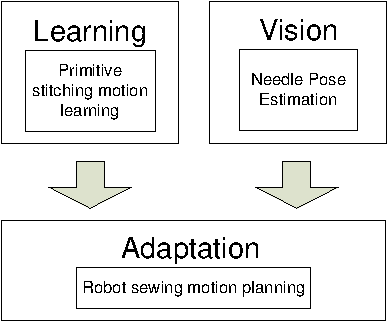
\includegraphics[width=5cm]{./fig/overview_single.pdf}
\caption{{System overview of stent graft sewing system. The robot is programmed by demonstrations. During task execution, the vision system estimate the needle pose and hence compute an adaptive trajectory for the sewing movements}}

\label{fig:overview}}

\end{figure}






